\documentclass[aspectratio=169]{beamer}

\usetheme{Madrid}
\usecolortheme{default}
\setbeamertemplate{navigation symbols}{}

\usepackage{graphicx}
\usepackage{tikz}
\usetikzlibrary{arrows.meta,positioning,shapes.geometric}
\usepackage{amsmath}
\usepackage{amssymb}
\usepackage{booktabs}
\usepackage{listings}
\usepackage{xcolor}
\usepackage{hyperref}

\graphicspath{{images/}}

\definecolor{codegray}{rgb}{0.95,0.95,0.95}

\lstdefinelanguage{Rust}{
  keywords={fn, let, mut, pub, impl, for, while, loop, match, if, else, use, mod, struct, enum, const, self, Self},
  sensitive=true,
  comment=[l]{//},
  morecomment=[s]{/*}{*/},
  morestring=[b]",
}

\lstset{
  language=Rust,
  backgroundcolor=\color{codegray},
  basicstyle=\ttfamily\tiny,
  keywordstyle=\color{blue},
  commentstyle=\color{gray},
  stringstyle=\color{orange},
  breaklines=true,
  breakatwhitespace=true,
  columns=fullflexible,
  frame=single,
  numbers=none,
  showstringspaces=false
}

\title[Lightweight Encryption]{Comparison of Lightweight Encryption Algorithms}
\subtitle{Progress Report - Phase 1}

\author[R. Jena, S. Kumar, P. Kumar]{
Rajesh Kumar Jena (B122088) \and
Soumil Kumar (B122114) \and
Punit Kumar (B422041)
}

\institute{
International Institute of Information Technology\\
Bhubaneswar\\
Supervisor: Prof. Debasish Jena
}

\date{March 2026}

\begin{document}

\begin{frame}
\titlepage
\end{frame}

\begin{frame}{Outline}
\tableofcontents
\end{frame}

\section{Introduction}

\begin{frame}{Motivation}
\begin{itemize}
    \item IoT deployments place cryptography on devices with limited CPU, memory, and energy
    \item Conventional algorithms are often too expensive for such platforms
    \item \textit{Lightweight cryptography} targets security with lower computational and memory cost
\end{itemize}
\end{frame}

\begin{frame}{Problem Statement and Objectives}
\textbf{Problem Statement}
\begin{itemize}
    \item AES, RSA, and ECC often exceed microcontroller resource limits
    \item Lightweight cryptography addresses this gap without sacrificing core security goals
\end{itemize}

\vspace{0.3cm}
\textbf{Objectives}
\begin{itemize}
    \item Implementation of lightweight ciphers (PRESENT, SPECK, ASCON) in Rust
    \item Benchmarking on Raspberry Pi Pico and host machine
    \item Performance analysis and comparison
    \item Security considerations for embedded systems
\end{itemize}
\end{frame}

\begin{frame}{Selected Algorithms}
\begin{itemize}
    \item \textbf{PRESENT}: Hardware-oriented 64-bit SPN cipher with 80/128-bit keys
    \item \textbf{SPECK}: Software-optimized ARX cipher (NSA-designed)
    \item \textbf{ASCON}: NIST Lightweight Cryptography Standard (2023) - authenticated encryption
\end{itemize}
\end{frame}

\section{Project Status}

\begin{frame}{Current Progress}
\small
\begin{tabular}{lll}
\toprule
Task & Status & Notes \\
\midrule
Literature Survey & Complete & 100\% \\
Algorithm Implementation & Complete & Core ciphers done \\
Test Vector Verification & Partial & Basic tests pass, KAT pending \\
Host Benchmarks & Partial & Initial metrics collected \\
Pico Hardware Benchmarks & Partial & Initial benchmarks run \\
ROM/RAM Analysis & Partial & Host analysis done \\
\bottomrule
\end{tabular}

\vspace{0.3cm}
\textbf{Completed:}
\begin{itemize}
    \item Rust implementations: PRESENT, SPECK, and ASCON
    \item Mode implementations: ECB, CBC, CTR for PRESENT and SPECK
    \item Embedded \texttt{no\_std} library for target hardware
    \item Basic validation: test vectors, consistency checks, ASCON tag verification
\end{itemize}

\vspace{0.2cm}
\textbf{Pending:}
\begin{itemize}
    \item NIST KAT tests, ROM/RAM analysis on Pico
    \item Energy consumption estimation
    \item Final report compilation
\end{itemize}
\end{frame}

\section{Implementation}

\begin{frame}[fragile]{PRESENT}
\begin{columns}
\begin{column}{0.42\textwidth}
\begin{itemize}
    \item 64-bit SPN block cipher
    \item 80-bit and 128-bit keys
    \item Designed for ultra-lightweight hardware
    \item Round steps: AddRoundKey, S-box, permutation
\end{itemize}
\end{column}
\begin{column}{0.58\textwidth}
\begin{lstlisting}
const SBOX: [u8; 16] = [
    0xC, 0x5, 0x6, 0xB, 0x9, 0x0, 0xA, 0xD,
    0x3, 0xE, 0xF, 0x8, 0x4, 0x7, 0x1, 0x2,
];

fn sbox_layer(state: u64) -> u64 {
    let mut result = 0u64;
    for i in 0..16 {
        let nibble = ((state >> (i * 4)) & 0xF) as usize;
        result |= u64::from(SBOX[nibble]) << (i * 4);
    }
    result
}
\end{lstlisting}
\end{column}
\end{columns}
\end{frame}

\begin{frame}[fragile]{SPECK}
\begin{columns}
\begin{column}{0.42\textwidth}
\begin{itemize}
    \item Software-optimized ARX cipher
    \item Feistel-like word-based structure
    \item Efficient on microcontrollers
\end{itemize}
\end{column}
\begin{column}{0.58\textwidth}
\begin{lstlisting}
pub enum SpeckVariant {
    Speck32_64,
    Speck48_72,
    Speck48_96,
    Speck64_96,
    Speck64_128,
}

impl SpeckVariant {
    pub const fn rounds(self) -> usize {
        match self {
            Self::Speck64_96 => 26,
            Self::Speck64_128 => 27,
            _ => 22,
        }
    }
}
\end{lstlisting}
\end{column}
\end{columns}
\end{frame}

\begin{frame}[fragile]{ASCON}
\begin{columns}
\begin{column}{0.42\textwidth}
\begin{itemize}
    \item NIST Lightweight Cryptography Standard (2023)
    \item Sponge-duplex construction
    \item 320-bit internal state
    \item Supports authenticated encryption and hashing
\end{itemize}
\end{column}
\begin{column}{0.58\textwidth}
\begin{lstlisting}
const ROUNDS_A: usize = 12;
const ROUNDS_B: usize = 6;

const fn p_sbox(s0: u64, s1: u64, s2: u64, s3: u64, s4: u64)
    -> (u64, u64, u64, u64, u64) {
    let s0 = s0 ^ s4;
    let s4 = s4 ^ s3;
    let s2 = s2 ^ s1;
    let t0 = (!s0) & s1;
    let t1 = (!s1) & s2;
    (s0, s1, s2, s3, s4)
}
\end{lstlisting}
\end{column}
\end{columns}
\end{frame}

\begin{frame}{Methodology}
\textbf{Evaluation Criteria}
\begin{itemize}
    \item \textbf{Execution Time}: ns per block (measured via hardware timer)
    \item \textbf{Cycles Per Byte (CPB)}: Platform-independent efficiency metric
    \item \textbf{Throughput}: Mbps for comparing speed
    \item \textbf{Memory}: ROM/RAM footprint analysis
\end{itemize}

\vspace{0.3cm}
\textbf{Hardware Platform}
\begin{itemize}
    \item Raspberry Pi Pico (ARM Cortex-M0+, 133 MHz, 264 KB SRAM)
    \item Rust \texttt{no\_std} embedded implementation
    \item Release mode with LTO and size optimization
\end{itemize}
\end{frame}

\begin{frame}{Benchmarking Approach}
\begin{itemize}
    \item Hardware timer for cycle-accurate measurements
    \item 1000+ iterations for statistical accuracy
    \item Warm-up runs before measurements
    \item Test vector validation for correctness
\end{itemize}
\end{frame}

\section{Results}

\begin{frame}{Benchmarks}
\small
\begin{tabular}{lrrrr}
\toprule
Algorithm & Platform & ns/block & CPB & Mbps \\
\midrule
PRESENT-80 & Host & 16,949 & 2,119 & 0.47 \\
PRESENT-80 & Pico & 23,665 & 2,958 & 0.34 \\
PRESENT-128 & Host & 16,990 & 2,124 & 0.47 \\
PRESENT-128 & Pico & 24,542 & 3,068 & 0.33 \\
SPECK-64/96 & Host & 246 & 31 & 32.52 \\
SPECK-64/96 & Pico & 336 & 42 & 23.81 \\
SPECK-64/128 & Host & 245 & 31 & 32.65 \\
SPECK-64/128 & Pico & 338 & 42 & 23.67 \\
ASCON-128 & Host & 1,518 & 95 & 10.54 \\
ASCON-128 & Pico & 2,117 & 132 & 7.56 \\
\bottomrule
\end{tabular}
\end{frame}

\begin{frame}{Visual Results: Block Cipher Comparison}
\centering
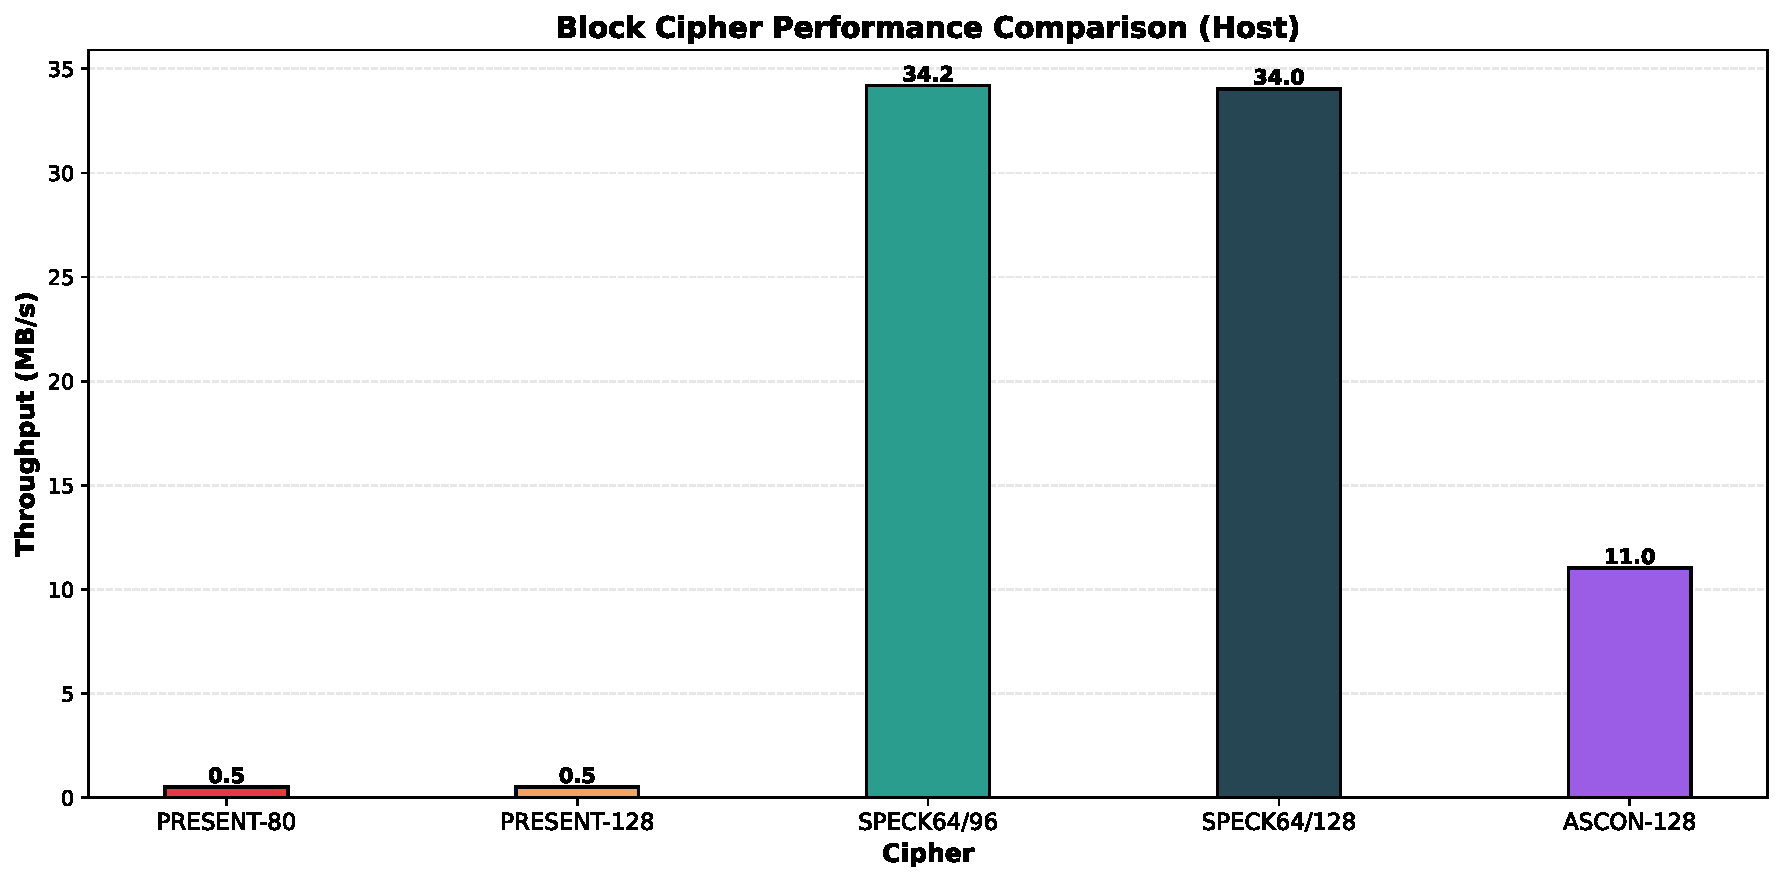
\includegraphics[width=0.92\textwidth]{block_cipher_comparison.pdf}
\end{frame}

\begin{frame}{Visual Results: Mode Comparison}
\centering
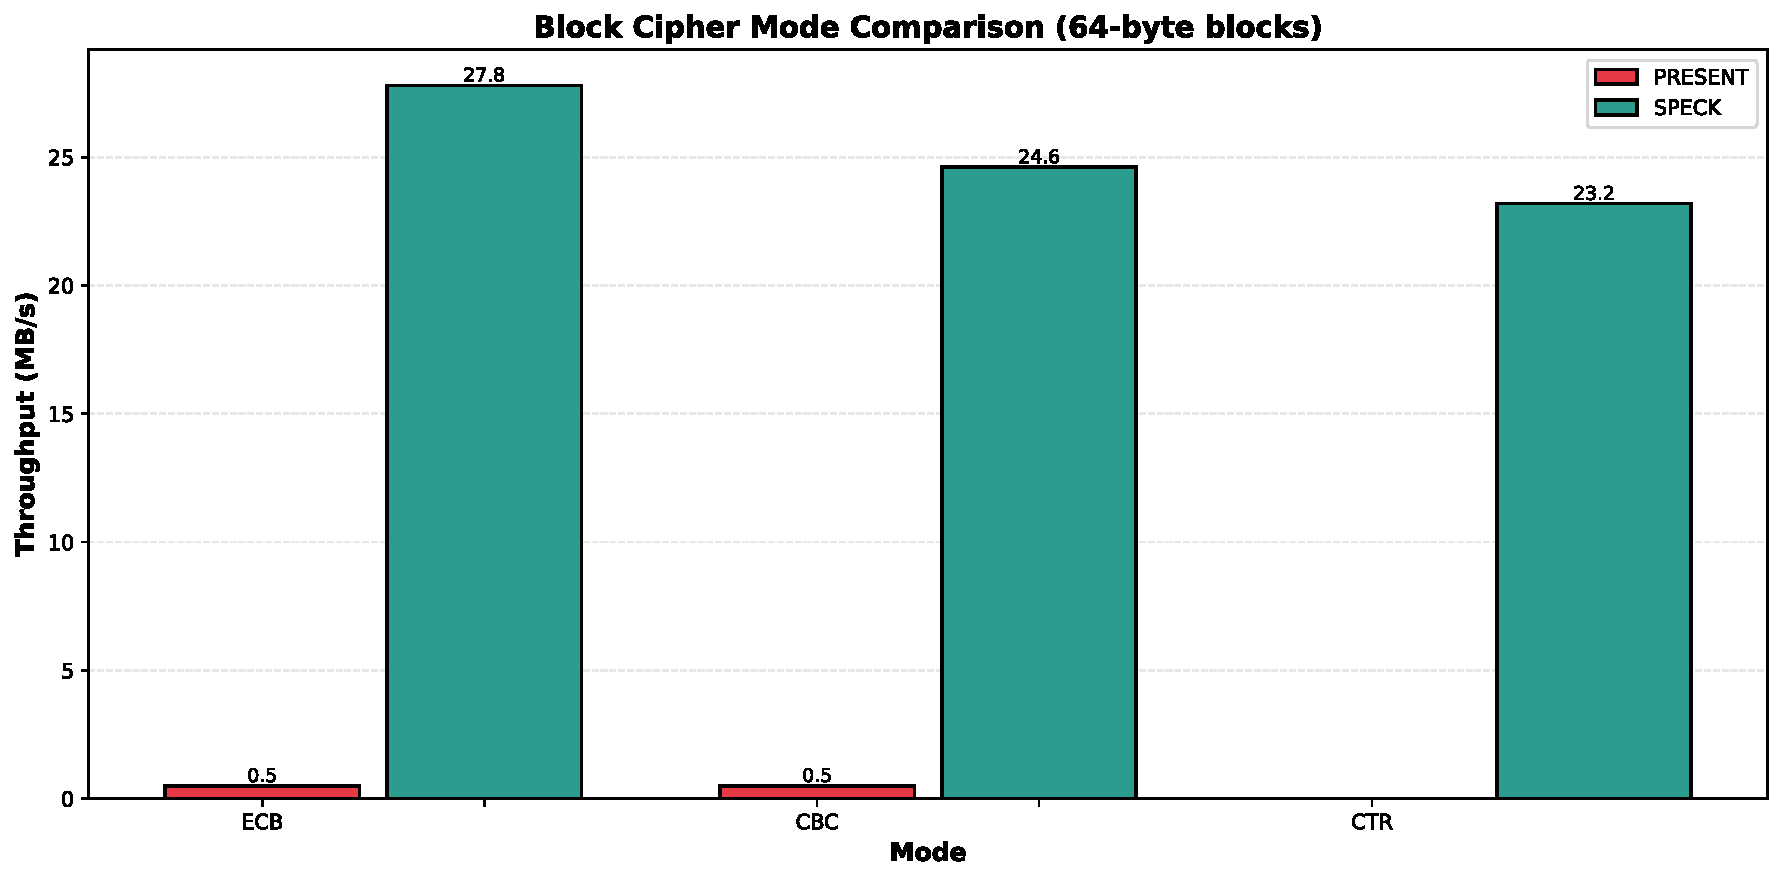
\includegraphics[width=0.92\textwidth]{mode_comparison.pdf}
\end{frame}

\begin{frame}{Visual Results: ASCON Phase Breakdown}
\centering
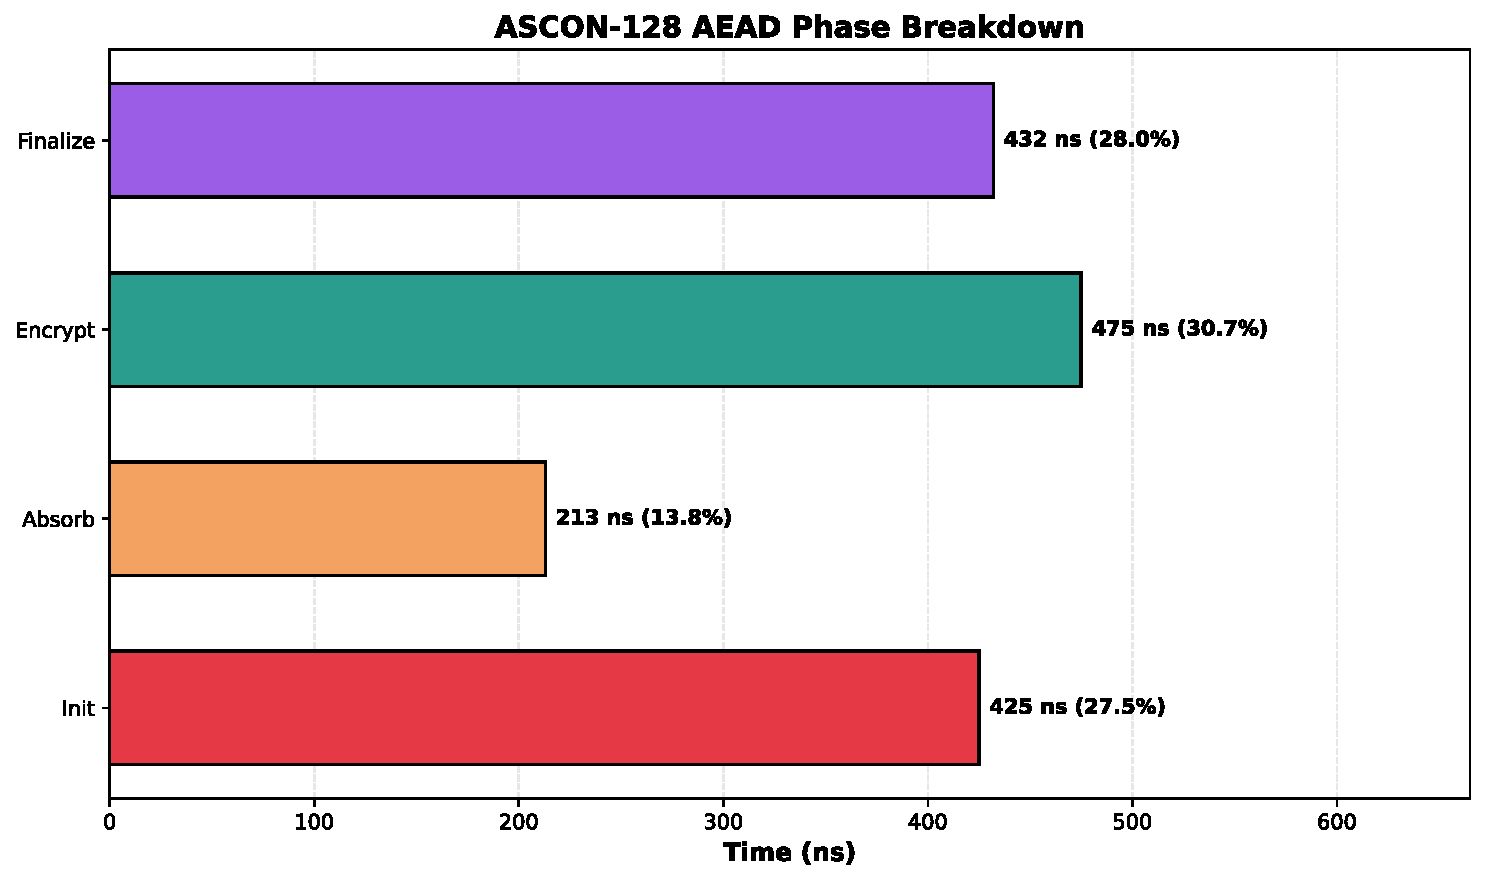
\includegraphics[width=0.92\textwidth]{ascon_breakdown.pdf}
\end{frame}

\begin{frame}{Visual Results: Scaling Analysis}
\centering
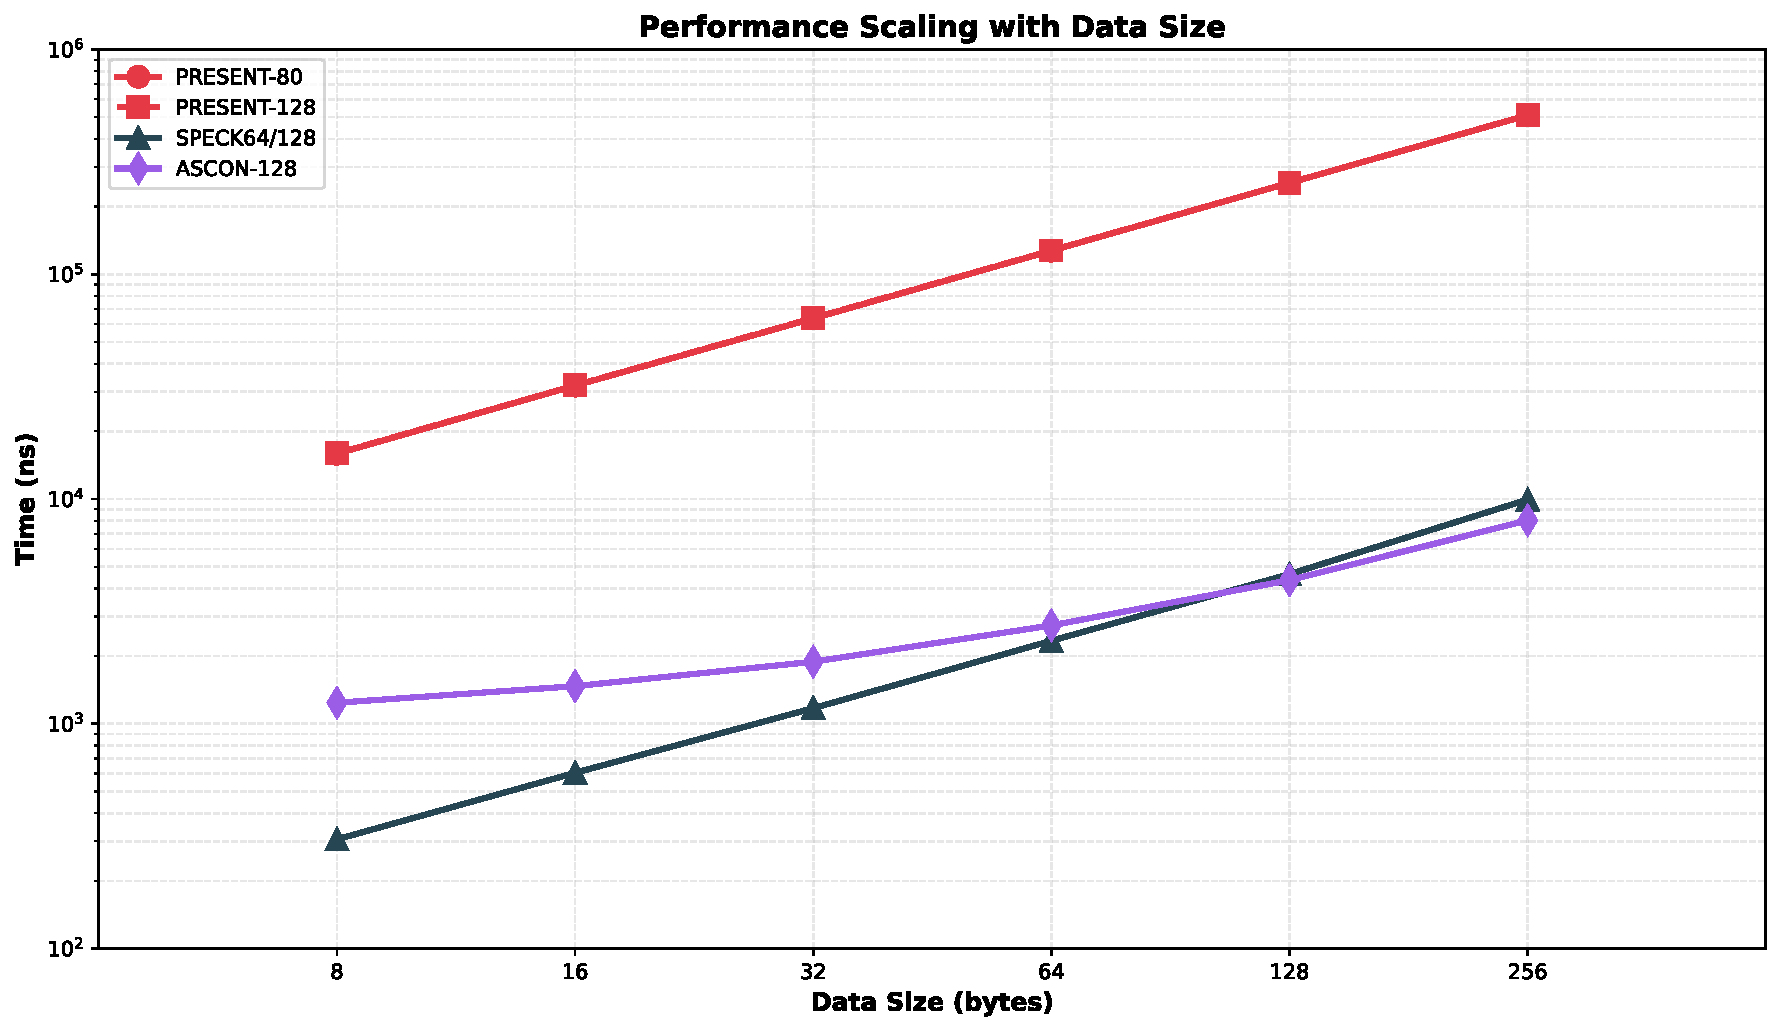
\includegraphics[width=0.92\textwidth]{scaling_analysis.pdf}
\end{frame}

\begin{frame}{Analysis}
\textbf{Performance Observations}
\begin{itemize}
    \item \textbf{SPECK} is the fastest: 23.67 Mbps on Pico, approximately 70x faster than PRESENT
    \item \textbf{ASCON} provides good balance with built-in authentication (7.56 Mbps on Pico)
    \item \textbf{PRESENT} is the slowest on software but designed for hardware efficiency
    \item CTR mode offers best performance among encryption modes for SPECK
    \item ASCON's initialization overhead is amortized over larger message sizes
\end{itemize}

\vspace{0.3cm}
\textbf{Memory Analysis}
\begin{itemize}
    \item \textbf{SPECK} has the smallest ROM footprint due to ARX-only operations (no lookup tables)
    \item \textbf{PRESENT} requires additional storage for S-box tables but remains compact
    \item \textbf{ASCON} has the largest code size due to 320-bit state and complex permutations
\end{itemize}
\end{frame}

\section{Conclusion}

\begin{frame}{Conclusion and Next Steps}
\textbf{Conclusion}
\begin{itemize}
    \item PRESENT, SPECK, and ASCON were evaluated using Rust-based implementations on Raspberry Pi Pico
    \item SPECK provides superior performance, PRESENT offers minimal memory footprint
    \item ASCON delivers strong modern security with functional completeness (NIST Standard 2023)
\end{itemize}

\vspace{0.3cm}
\textbf{Short-Term Next Steps}
\begin{itemize}
    \item NIST KAT Tests: Integrate official Known Answer Test vectors
    \item Code Size Analysis: Static analysis for .text/.data/.bss sections
    \item Statistical Rigor: Report median/min/max across multiple runs
\end{itemize}

\vspace{0.2cm}
\textbf{Medium-Term Next Steps}
\begin{itemize}
    \item FELICS Comparison: Compare against established lightweight crypto benchmarks
    \item SUPERCOP-Style Timing: Implement cycle-accurate benchmarking
    \item Side-Channel Discussion: Analyze timing attack resistance for ARX ciphers
\end{itemize}
\end{frame}

\begin{frame}
\Huge Thank You\\
\vspace{0.5cm}
\end{frame}

\end{document}
